% Recipe: xelatex -> bibtex -> xelatex*2
\documentclass{article}
\usepackage{amsmath} % Math Symbols & Equations
\usepackage{amssymb} % Special Math Symbols
\usepackage{graphicx} % Graphics & Images
\usepackage{hyperref} % Hypertext Link
\usepackage{syntonly} % Syntax Check Only
\usepackage{textcomp} % Special Symbols
\usepackage{verbatim} % Long Comments
% \syntaxonly
\hyphenation{}
\hypersetup{colorlinks}
\title{\LaTeX{} Examples}
\author{GasinAn}
\begin{document}
    \maketitle
    Here are examples of using \LaTeX{}!
    \section{Basics}
    \subsection{Paragraphs}
    This sentence is in the 1st paragraph.
    This sentence is also in the 1st paragraph.

    This sentence is in the 2nd paragraph.
    \subsection{Special Characters}
    \~ \# \$ \% \^ \& \_ \{ \} \\ % Wrong!
    \~{} \# \$ \% \^{} \& \_ \{ \} \\ \textbackslash % Right!
    \section{Typesetting}
    \subsection{Line Breaking}
    This sentence is in the 1st line.\\
    This sentence is in the 2nd line.\newline
    This sentence is in the 3rd line.
    \subsection{Page Breaking}
    This sentence is in the 1st page.\newpage
    This sentence is in the 2nd page.
    \subsection{Quotation Marks}
    'Wrong' "Wrong"\\
    `Right' ``Right''
    \subsection{Dashes}
    X-ray\\
    Page 0--65535\\
    Yes---or no?\\
    $-2147483648$
    \subsection{Tilde}
    This is not good.\~{}\\
    This is good!$\sim$
    \subsection{Degree Symbol}
    $361^{\circ}$\\
    $-273.15^{\circ}\mathrm{C}$ (Better: $-273.15\,^{\circ}\mathrm{C}$)\\
    $-273.15$ \textcelsius{} = $-459.67$ \textdegree{}F
    \subsection{Ellipsis}
    This is not good...\\
    This is good!\dots\\
    This is also good!\ldots
    \subsection{Special Letters}
    Hello everyone, I am Schr\"odinger, and here are my brothers:
    Schr\.odinger, Schr\=odinger, Schr\~odinger,
    Schr\^odinger, Schr\'odinger, Schr\`odinger,
    Schr\u odinger, Schr\v odinger and Schr\H odinger.
    Do you know about angstrom? Its symbol is \AA.
    \subsection{The Space Between Words}
    Mr. An do not hate FORTRAN. However you may hate it. (Bad!)\\
    Mr.~An do not hate FORTRAN\@. However you may hate it. (Good!)
    \subsection{Cross References}\label{ref}
    A reference to this subsection looks like:
    ``see subsection~\ref{ref} on page~\pageref{ref}.''
    \subsection{Footnotes}
    Footnotes referring to a sentence or part of it showld be put
    after the comma or period.\footnote{This is a footnote.}
    \subsection{Emphasized Words}
    emphasis emphasis \underline{emphasis} emphasis emphasis\\
    \textit{emphasis emphasis \underline{emphasis} emphasis emphasis}\\
    emphasis emphasis \emph{emphasis} emphasis emphasis\\
    \textit{emphasis emphasis \emph{emphasis} emphasis emphasis}
    \subsection{Itemize}
    Here is an example of itemize:
    \begin{itemize}
        \item John Higgins
        \item Mark Williams
        \item Ronnie O'Sullivan
    \end{itemize}
    \subsection{Enumerate}
    Here is an example of enumerate:
    \begin{enumerate}
        \item World Championship
        \item UK Championship
        \item Masters
    \end{enumerate}
    \subsection{Description}
    Here is an example of description:
    \begin{description}
        \item[Topspin] striking the white ball above the midpoint of its
        vertical plane as it faces the shooter quickly, and after the white
        ball hits the colour ball, the included angle between the shift
        directions of two balls is less than 90\textdegree{}.
        \item[Stun] striking the white ball at the midpoint of its vertical
        plane as it faces the shooter quickly, and after the white ball hits
        the colour ball, the included angle between the shift directions of two
        balls is 90\textdegree{}.
        \item[Screw] striking the white ball below the midpoint of its vertical
        plane as it faces the shooter quickly, and after the white ball hits
        the colour ball, the included angle between the shift directions of two
        balls is more than 90\textdegree{}.
    \end{description}
    \subsection{Quote}
    Here is an example of quote:
    \begin{quote}
        \dots lensed FRBs, as a powerful probe and completely independent
        dataset based on a different physical phenomenon, would provide
        complementary information and therefore are of vital importance to
        clarify the tension between the latest Planck-inferred $H_0$ and the
        one from direct local distance ladder observations.\footnote{
            Li, ZX., Gao, H., Ding, XH. \textit{et al}. Strongly lensed
            repeating fast radio bursts as precision probes of the universe.
            \textit{Nat Commun} \textbf{9}, 3833 (2018).}
    \end{quote}
    \subsection{Abstract}
    Here is an example\footnote{
        Lin, L., Zhang, C.F., Wang, P. \textit{et al}.
        No pulsed radio emission during a bursting phase of a Galactic magnetar.
        \textit{Nature} \textbf{587}, 63–65 (2020).} of abstract:
    \begin{abstract}
        Fast radio bursts (FRBs) are millisecond-duration radio transients of
        unknown physical origin observed at extragalactic distances. It has
        long been speculated that magnetars are the engine powering repeating
        bursts from FRB sources, but no convincing evidence has been collected
        so far. Recently, the Galactic magnetar SRG 1935+2154 entered an active
        phase by emitting intense soft $\gamma$-ray bursts. One FRB-like event
        with two peaks (FRB 200428) and a luminosity slightly lower than the
        faintest extragalactic FRBs was detected from the source, in
        association with a soft $\gamma$-ray/hard-X-ray flare. Here we report
        an eight-hour targeted radio observational campaign comprising four
        sessions and assisted by multi-wavelength (optical and hard-X-ray)
        data. During the third session, 29 soft-$\gamma$-ray repeater (SGR)
        bursts were detected in $\gamma$-ray energies. Throughout the observing
        period, we detected no single dispersed pulsed emission coincident with
        the arrivals of SGR bursts, but unfortunately we were not observing
        when the FRB was detected. The non-detection places a fluence upper
        limit that is eight orders of magnitude lower than the fluence of FRB
        200428. Our results suggest that FRB–SGR burst associations are rare.
        FRBs may be highly relativistic and geometrically beamed, or FRB-like
        events associated with SGR bursts may have narrow spectra and
        characteristic frequencies outside the observed band. It is also
        possible that the physical conditions required to achieve coherent
        radiation in SGR bursts are difficult to satisfy, and that only under
        extreme conditions could an FRB be associated with an SGR burst.
    \end{abstract}
    \newpage
    \subsection{Printing Verbatim}
\begin{verbatim}
program hellolatex
print *, "Hello, LaTeX!"
end program hellolatex
\end{verbatim}
\begin{verbatim*}
      PROGRAM HELLOLATEX
      PRINT *, 'HELLO, LATEX.'
      END PROGRAM HELLOLATEX
\end{verbatim*}
    The last line of the program can also be \verb|end| (or \verb*|      END|).
    \subsection{Table}
    \begin{table}[htbp]
        \def\bs{$\bigstar$} % Define a new command!
        \centering
        \begin{tabular}{c|cccccc}
            \hline
            Year & Jan. & Mar. & May & July & Sept. & Nov. \\
            \hline
            2002 &      &      &     &      &       & \bs  \\
            2003 & \bs  &      & \bs &      & \bs   &      \\
            2004 & \bs  & \bs  & \bs & \bs  &       & \bs  \\
            2005 & \bs  & \bs  & \bs & \bs  & \bs   & \bs  \\
            2006 &      & \bs  &     & \bs  & \bs   & \bs  \\
            2007 & \bs  &      &     & \bs  &       &      \\
            2008 &      & \bs  &     &      &       &      \\
            2009 & \bs  &      &     &      & \bs   &      \\
            2010 & \bs  &      &     &      &       &      \\
            \hline
        \end{tabular}
        \caption{Top Division Champion Record of Asash\=ory\=u Akinori}
        \label{table} % Put \label here!
    \end{table}
    \subsection{Figure}
    \begin{figure}[htbp]
        \centering
        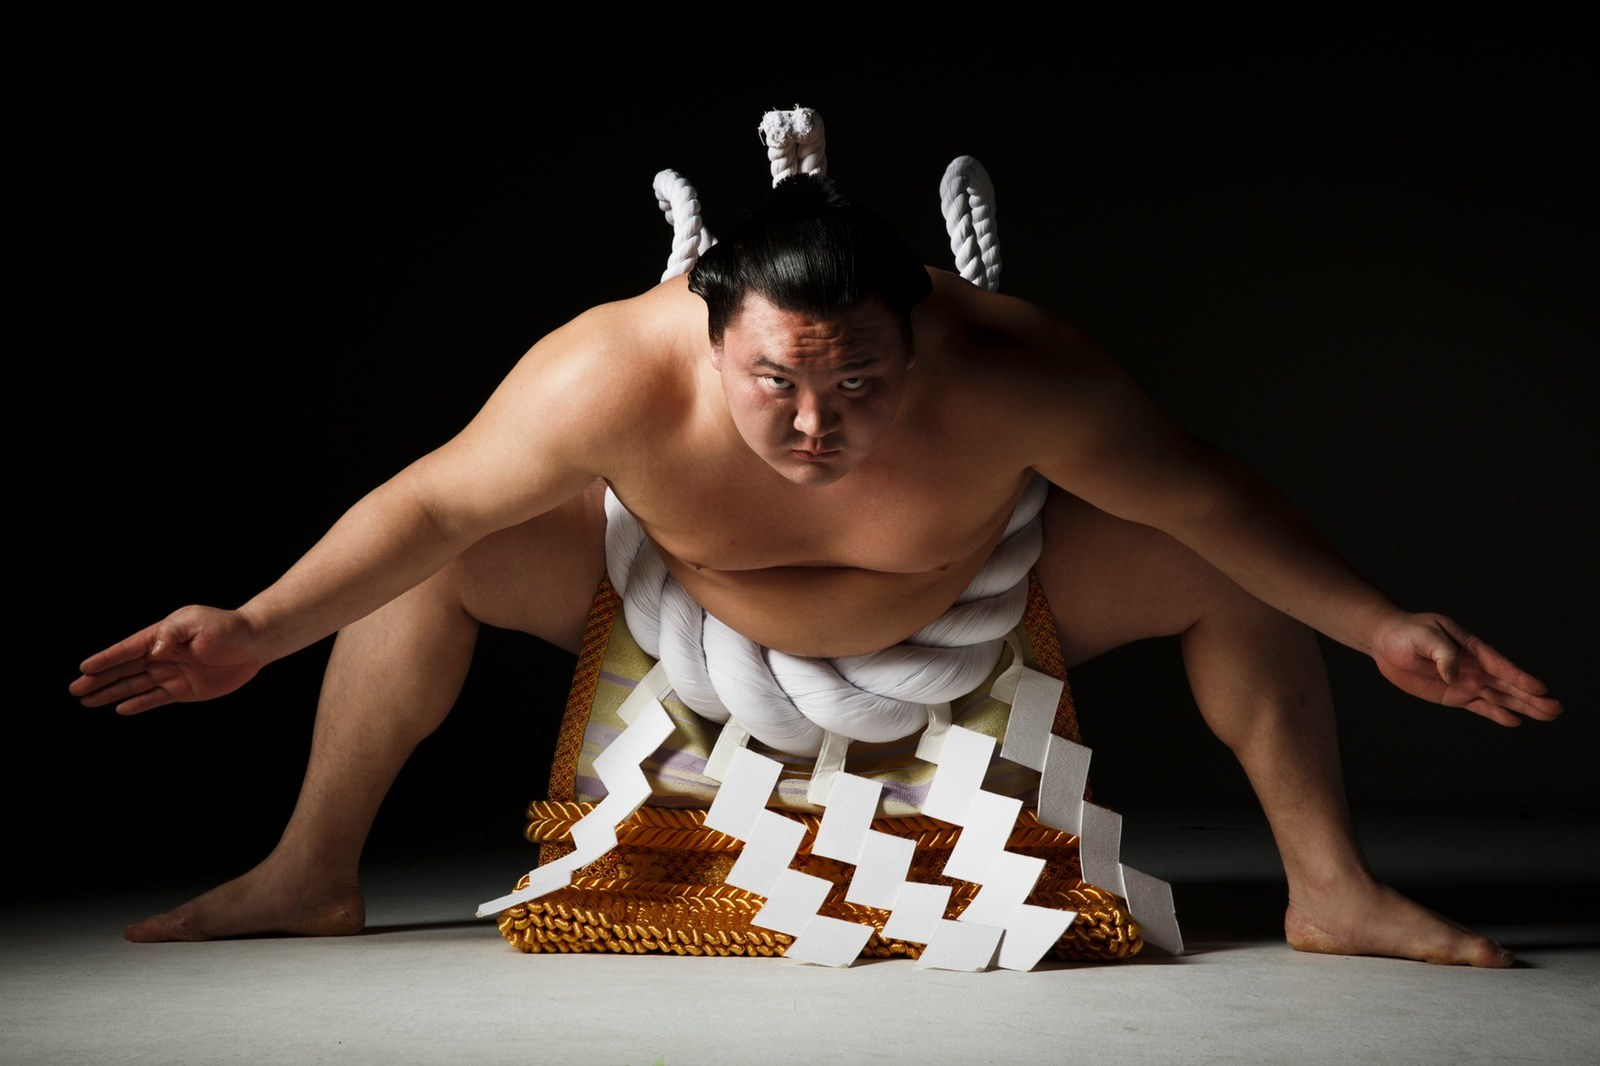
\includegraphics[width=0.6\textwidth]{img/Hakuho.jpg}
        \caption{Hakuh\=o Sh\=o}
        \label{figure} % Put \label here!
    \end{figure}
    \section{Typesetting Mathematical Formulae}
    \subsection{Single Euations}
    Show equation $E=mc^1$ in display style:
    \begin{equation*}
        E=mc^1.
    \end{equation*}
    Show equation $E=mc^2$ in display style with a tag:
    \begin{equation}
        E=mc^2. \label{eq2}
    \end{equation}
    Show equation $E=mc^3$ in display style with a specific tag:
    \begin{equation}
        E=mc^3. \tag{$\ast$} \label{eq3}
    \end{equation}
    Equation~\eqref{eq2} is right, while equation~\eqref{eq3} is wrong!
    \subsection{Texts}
    This is wrong:
    \begin{equation*}
        x > 0    for all x \in R_+.
    \end{equation*}
    This is right:
    \begin{equation*}
        x > 0 \qquad \text{for all } x \in \mathbb{R_+}.
    \end{equation*}
    \subsection{Superscripts and Subscripts}
    $ \sum_{i=1}^{100} i = \sum^{100}_{j=1} j $.
    $ a^x+y \neq a^{x+y} $.
    $ e^{x^2} \neq {e^x}^2 $.
    \subsection{Root Signs}
    $ \sqrt{5} > \sqrt[5]{5} $.
    \subsection{Names of Functions}
    This is wrong:
    $ 2 \text{lim}_{x \rightarrow \infty} \text{arctan} x = \pi $.\\
    This is right:
    $ 2 \lim_{x \rightarrow \infty} \arctan x = \pi $.
    \subsection{Modulo}
    $ 5 \bmod 2 = 1$, $ 5 \equiv 1 \pmod{2}$.
    \subsection{Fraction}
    $\frac{\mathrm{d}^{n}y}{\mathrm{d}x^{n}}$.
    $\frac{\partial^{2}z}{\partial{x}\partial{y}}$.
    \subsection{Binomial Coefficient}
    $ \binom{n}{k} = \binom{n-1}{k} + \binom{n-1}{k-1}$.
    \subsection{Stacking Symbols}
    $ 2\text{K}\text{Mn}\text{O}_4 \stackrel{\triangle}{\longrightarrow}
      \text{K}_2\text{Mn}\text{O}_4+\text{Mn}\text{O}_2+\text{O}_2\uparrow $,
    $ 2\text{H}_2\text{O}_2 \xrightarrow[]{\text{Mn}\text{O}_2}
    2\text{H}_2\text{O}+\text{O}_2\uparrow $.\\
    The second one is better!\\
    Math is much more complex than chemistry:
    \begin{equation*}
        \sum_{\substack{1\le{i}\le{n}\\j>i}} l_{ij}^2 = 0.
    \end{equation*}
    \subsection{Aligning}
    \begin{align}
        \nabla\frac{1}{r} & = \nabla\frac{1}{\sqrt{x^2+y^2+z^2}} \label{oeq}\\
            & = -\frac{x\boldsymbol{i}+y\boldsymbol{j}+z\boldsymbol{k}}
                      {\sqrt{x^2+y^2+z^2}^3} \nonumber \\
            & = -\frac{\hat{\boldsymbol{r}}}{r^2}. \tag{$\star$} \label{beq}
    \end{align}
    \eqref{oeq} can be derived by definition,
    and the result \eqref{beq} is beautiful!
    \subsection{Matrices}
    \begin{equation*}
        \boldsymbol{I} = 
        \begin{bmatrix}
            1 & 0 \\
            0 & 1
        \end{bmatrix}.
    \end{equation*}
    \subsection{Piecewise Functions}
    \begin{equation*}
        |x| = 
        \begin{cases}
            -x & \text{if } x < 0, \\
             0 & \text{if } x = 0, \\
             x & \text{if } x > 0. \\
        \end{cases}
    \end{equation*}
    \subsection{Spacing}
    $ \text{This is} \  \text{a space.} $ \\
    $ \text{This is} \! \text{-3/18 quad.} $ \\
    $ \text{This is} \, \text{3/18 quad.} $ \\
    $ \text{This is} \: \text{4/18 quad.} $ \\
    $ \text{This is} \; \text{5/18 quad.} $ \\
    $ \text{This is} \quad \text{1 quad.} $ \\
    $ \text{This is} \qquad \text{2 quads.} $
    \subsection{Phantoms}
    This is wrong: ${}^{99}_{ 9}\text{C}R_{abc}^{   d}$.\\
    This is also wrong: ${}^{99}_{\ 9}\text{C}R_{abc}^{\ \ \ d}$.\\
    This is right: ${}^{99}_{\phantom{9}9}\text{C}R_{abc}^{\phantom{abc}d}$.
    \subsection{List of Symbols}
    See \href{https://www.ctan.org/tex-archive/info/symbols/comprehensive}{The Comprehensive \LaTeX{} Symbol List} for many many symbols!
    \begin{table}[!htbp]
        \centering
        \begin{tabular}{cccccc}
            $\dot{a}$ & \verb|\dot{a}| &
            $\bar{a}$ & \verb|\bar{a}| &
            $\hat{a}$ & \verb|\hat{a}| \\
            $\ddot{a}$ & \verb|\ddot{a}| &
            $\vec{a}$ & \verb|\vec{a}| \\
        \end{tabular}
    \end{table}
    \begin{table}[!htbp]
        \centering
        \begin{tabular}{cccccc}
            $<$ & \verb|<| &
            $>$ & \verb|>| &
            $=$ & \verb|=| \\
            $\leq$ & \verb|\leq| &
            $\geq$ & \verb|\geq| &
            $\equiv$ & \verb|\equiv| \\
            $\ll$ & \verb|\ll| &
            $\gg$ & \verb|\gg| \\
            $\in$ & \verb|\in| &
            $\ni$ & \verb|\ni| &
            $\sim$ & \verb|\sim| \\
            $\subset$ & \verb|\subset| &
            $\supset$ & \verb|\supset| &
            $\simeq$ & \verb|\simeq| \\
            $\subseteq$ & \verb|\subseteq| &
            $\supseteq$ & \verb|\supseteq| &
            $\approx$ & \verb|\approx| \\
            $:$ & \verb|:| &
            $\mid$ & \verb|\mid| &
            $\propto$ & \verb|\propto| \\
            $\perp$ & \verb|\perp| &
            $\parallel$ & \verb|\parallel| \\
            $\not\in$ & \verb|\not\in| &
            $\not\ni$ & \verb|\not\ni| &
            $\neq$ & \verb|\neq| \\
            $\not\subset$ & \verb|\not\subset| &
            $\not\supset$ & \verb|\not\supset| &
            $\not\equiv$ & \verb|\not\equiv| \\
            $\not\subseteq$ & \verb|\not\subseteq| &
            $\not\supseteq$ & \verb|\not\supseteq| \\
        \end{tabular}
    \end{table}
    \begin{table}[!htbp]
        \centering
        \begin{tabular}{cccccccc}
            $+$ & \verb|+| &
            $-$ & \verb|-| &
            $\times$ & \verb|\times| &
            $\div$ & \verb|\div| \\
            $\pm$ & \verb|\pm| &
            $\mp$ & \verb|\mp| &
            $\cdot$ & \verb|\cdot| &
            $/$ & \verb|/| \\
            $\cup$ & \verb|\cup| &
            $\cap$ & \verb|\cap| &
            $\oplus$ & \verb|\oplus| &
            $\otimes$ & \verb|\otimes| \\
            $\star$ & \verb|\star| &
            $\ast$ & \verb|\ast| &
            $\dagger$ & \verb|\dagger| &
            $\ddagger$ & \verb|\ddagger| \\
        \end{tabular}
    \end{table}
    \begin{table}[!htbp]
        \centering
        \begin{tabular}{cccccccc}
            $\sum$ & \verb|\sum| &
            $\prod$ & \verb|\prod| &
            $\bigcup$ & \verb|\bigcup| &
            $\bigcap$ & \verb|\bigcap| \\
            $\int$ & \verb|\int| &
            $\oint$ & \verb|\oint| &
            $\bigoplus$ & \verb|\bigoplus| &
            $\bigotimes$ & \verb|\bigotimes| \\
        \end{tabular}
    \end{table}
    \begin{table}[!htbp]
        \centering
        \begin{tabular}{cccc}
            $\leftarrow$ & \verb|\leftarrow| &
            $\longleftarrow$ & \verb|\longleftarrow| \\
            $\rightarrow$ & \verb|\rightarrow| &
            $\longrightarrow$ & \verb|\longrightarrow| \\
            $\leftrightarrow$ & \verb|\leftrightarrow| &
            $\longleftrightarrow$ & \verb|\longleftrightarrow| \\
            $\Leftarrow$ & \verb|\Leftarrow| &
            $\Longleftarrow$ & \verb|\Longleftarrow| \\
            $\Rightarrow$ & \verb|\Rightarrow| &
            $\Longrightarrow$ & \verb|\Longrightarrow| \\
            $\Leftrightarrow$ & \verb|\Leftrightarrow| &
            $\Longleftrightarrow$ & \verb|\Longleftrightarrow| \\
            $\mapsto$ & \verb|\mapsto| &
            $\longmapsto$ & \verb|\longmapsto| \\
            $\uparrow$ & \verb|\uparrow| &
            $\downarrow$ & \verb|\downarrow| \\
        \end{tabular}
    \end{table}
    \begin{table}[!htbp]
        \centering
        \begin{tabular}{cccc}
            $\overleftarrow{AB}$ & \verb|\overleftarrow{AB}| &
            $\underleftarrow{AB}$ & \verb|\underleftarrow{AB}| \\
            $\overrightarrow{AB}$ & \verb|\overrightarrow{AB}| &
            $\underrightarrow{AB}$ & \verb|\underrightarrow{AB}| \\
            $\overleftrightarrow{AB}$ & \verb|\overleftrightarrow{AB}| &
            $\underleftrightarrow{AB}$ & \verb|\underleftrightarrow{AB}| \\
        \end{tabular}
    \end{table}
    \begin{table}[!htbp]
        \centering
        \begin{tabular}{cccc}
            $(a)$ & \verb|(a)| &
            $[a]$ & \verb|[a]| \\
            $\{a\}$ & \verb|\{a\}| &
            $\langle{a}\rangle$ & \verb|\langle{a}\rangle| \\
            $\lfloor{a}\rfloor$ & \verb|\lfloor{a}\rfloor| &
            $\lceil{a}\rceil$ & \verb|\lceil{a}\rceil| \\
            $\lvert{a}\rvert$ & \verb|\lvert{a}\rvert| &
            $\lVert{a}\rVert$ & \verb|\lVert{a}\rVert| \\
        \end{tabular}
    \end{table}
    \begin{table}[!htbp]
        \centering
        \begin{tabular}{cccccccc}
            $\ldots$ & \verb|\ldots| &
            $\cdots$ & \verb|\cdots| &
            $\vdots$ & \verb|\vdots| &
            $\ddots$ & \verb|\ddots| \\
            $\because$ & \verb|\because| &
            $\therefore$ & \verb|\therefore| &
            $\infty$ & \verb|\infty| &
            $\%$ & \verb|\%| \\
            $\nabla$ & \verb|\nebla| &
            $\angle$ & \verb|\angle| &
            $\square$ & \verb|\square| &
            $\varnothing$ & \verb|\varnothing| \\
            $\hbar$ & \verb|\hbar| &
            $\ell$ & \verb|\ell| &
            $\Re$ & \verb|\Re| &
            $\Im$ & \verb|\Im| \\
            $\forall$ & \verb|\forall| &
            $\exists$ & \verb|\exists| &
            $\aleph$ & \verb|\aleph| &
            $\partial$ & \verb|\partial| \\
            $\S$ & \verb|\S| &
            $\P$ & \verb|\P| \\
        \end{tabular}
    \end{table}
    \section{Bibliography}
    Fast radio bursts (FRBs) are millisecond-duration bright radio transients
    \cite{Li2018,Lin2020}.
    \bibliographystyle{abbrv}
    \bibliography{astro}
    \section{New Commands}
    \newcommand{\isgood}[3][good]{\href{#3}{\emph{#2}} is #1!}
    \isgood{Lshort}{https://www.ctan.org/pkg/lshort}\\
    \isgood[also good]{Lnotes}{https://github.com/huangxg/lnotes}
    \section{Hypertext Links}
    Want to make \href{lexample.pdf}{\emph{\LaTeX{} Examples}} better?\\
    Start pull requests or issues on
    \href{https://github.com/GasinAn/lexamples}{Github},
    or send emails to
    \href{mailto:Gasin185@163.com}{Gasin185@163.com}!
\end{document}
